\documentclass[main.tex]{subfiles}
\begin{document}
\section{Analysis}
From the output of a single block encrypted with AES, we can see that the
algorithm has strong confusion and diffusion properties. Even single bit changes
in the key or the plaintext result in a significantly different ciphertext.

It is also observed that the \texttt{subBytes} (substitution) step of the
encryption algorithm ensures that an all-zero key and message do not lead to an
all-zero ciphertext showing that the algorithm is not linear in its inputs.

\lstinputlisting[style=codeStylePy3]{aes.py}
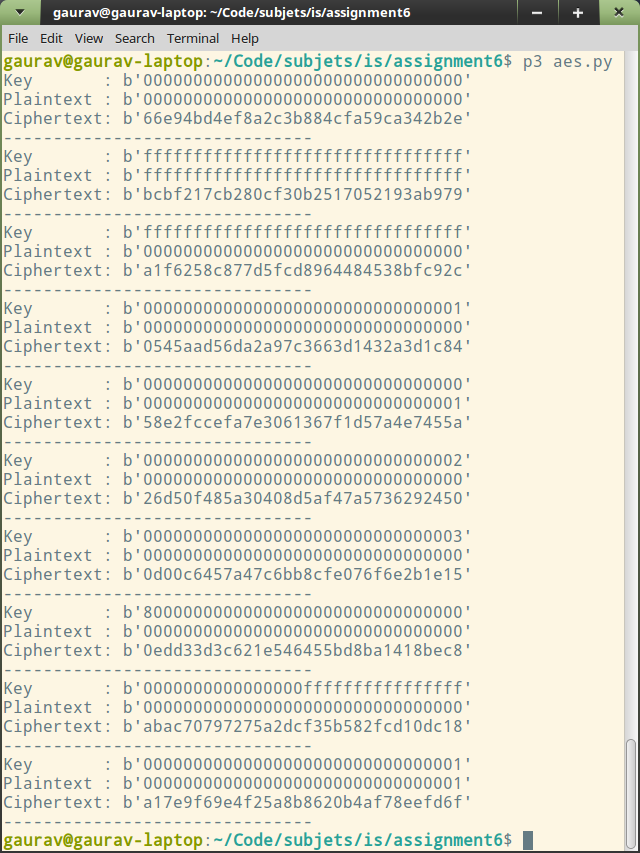
\includegraphics[width=\textwidth]{output.png}

\lstinputlisting[style=codeStylePy3]{aes_timing.py}
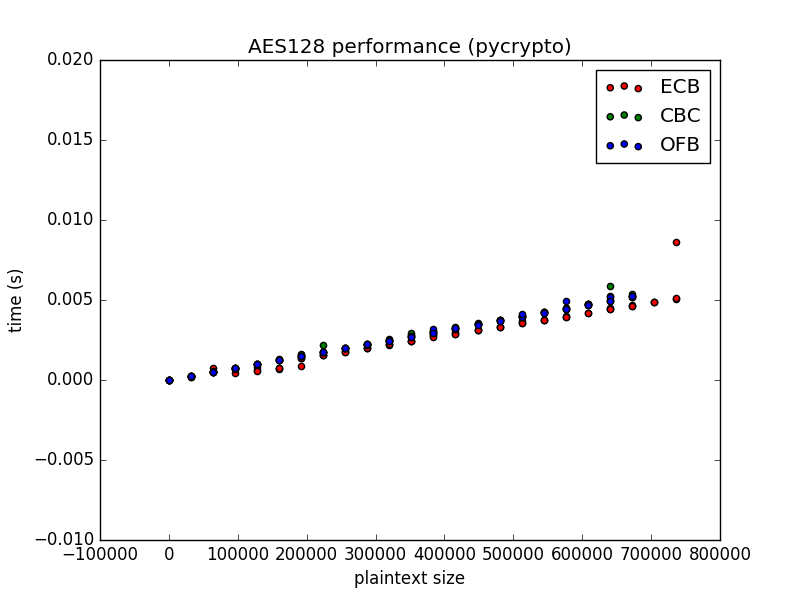
\includegraphics[width=\textwidth]{plot.png}

The plot shows that the execution time varies linearly with the input size, and
is not highly dependent on the mode of operation.


\end{document}
